% 第5章第3节：变量消元（消元操作与不变量、中间函数与填充边、消元次序与计算开销）。

\section{变量消元}
\label{sec:graph-variable-elimination}

链和树上的递推每次处理一个端点：把只连着已处理部分的变量汇总掉，留下一张接口表。一般依赖图可能有环，局部函数也可能读取三个以上变量，这时不一定存在只连着一个邻居的变量。本节把“汇总一个变量”写成对局部函数集合的一般操作，说明按任意次序逐个汇总都给出正确的最优值；随后会看到，正确性不依赖次序，中间表的大小却依赖次序。

本节沿用第~\ref{sec:graph-local-functions}节的四变量例子：二值变量$x_1,\ldots,x_4$，两个三元局部函数$\phi_A(x_1,x_2,x_3)$与$\phi_B(x_2,x_3,x_4)$，总成本$F=\phi_A+\phi_B$。两张表由表~\ref{tab:graph-dp-ternary-tables}给出，其中$+\infty$表示禁止的组合。

\begin{table}[!htb]
  \centering
  \caption{四变量例子的两个三元局部函数。第一列的三位二进制串对$\phi_A$表示$(x_1,x_2,x_3)$，对$\phi_B$表示$(x_2,x_3,x_4)$。}
  \label{tab:graph-dp-ternary-tables}
  \begin{tabular}{ccccccccc}
    \toprule
    取值 & $000$ & $001$ & $010$ & $011$ & $100$ & $101$ & $110$ & $111$\\
    \midrule
    $\phi_A(x_1,x_2,x_3)$ & $1$ & $0$ & $2$ & $+\infty$ & $0$ & $2$ & $1$ & $2$\\
    $\phi_B(x_2,x_3,x_4)$ & $2$ & $1$ & $0$ & $+\infty$ & $+\infty$ & $0$ & $1$ & $2$\\
    \bottomrule
  \end{tabular}
\end{table}

\subsection{消元操作}

\paragraph{汇总一个变量}
设当前有一组局部函数$\mathcal F$，总成本是它们的和。要汇总变量$x_i$，先找出所有作用域含$i$的函数，记为$\mathcal F_i$；它们的作用域之并去掉$i$，记为$R_i$。固定$R_i$中变量的取值后，把$\mathcal F_i$中的函数相加，再对$x_i$取最小，得到一个新函数
\begin{equation}
\psi_i(\bm x_{R_i})=\min_{x_i\in\mathcal X_i}\sum_{f\in\mathcal F_i}f .
\label{eq:graph-dp-elimination-step}
\end{equation}
然后从$\mathcal F$中删去$\mathcal F_i$，加入$\psi_i$；不含$i$的函数保持原样。这一操作称为消去$x_i$，逐个消去变量的方法称为\term{变量消元}（variable elimination）。链上的$m_{1\to2}$正是消去$x_1$时得到的新函数。

在四变量例子中消去$x_1$：只有$\phi_A$含$1$，$R_1=\{2,3\}$。对$(x_2,x_3)=(0,0),(0,1),(1,0),(1,1)$，分别比较$x_1=0,1$两行，得到
\[
\psi_1(x_2,x_3)=\bigl(\min(1,0),\ \min(0,2),\ \min(2,1),\ \min(+\infty,2)\bigr)=(0,\,0,\,1,\,2),
\]
达到最小值的$x_1$依次为$1,0,1,1$。消元后的函数集合是$\{\psi_1,\phi_B\}$。可以逐项核对它没有改变剩余变量的最优成本：例如取$(x_2,x_3,x_4)=(1,0,1)$，原问题对$x_1$求最小值为$\min\bigl(\phi_A(0,1,0)+\phi_B(1,0,1),\ \phi_A(1,1,0)+\phi_B(1,0,1)\bigr)=\min(2,1)=1$，新集合给出$\psi_1(1,0)+\phi_B(1,0,1)=1+0=1$，两者相同。

\paragraph{不变量与正确性}
上面的核对对每个剩余配置都成立，这不是巧合。设已经按某个次序消去了下标集合$Z$中的变量，把剩余变量的一个配置记为$\bm y=\bm x_{V\setminus Z}$。消元过程保持下面的不变量：
\begin{equation}
\sum_{f\in\mathcal F}f(\bm y)=\min_{\bm x_Z}F(\bm x_Z,\bm y)\qquad\text{对每个剩余配置}\ \bm y .
\label{eq:graph-dp-elimination-invariant}
\end{equation}

\begin{theorem}[变量消元的正确性]
\label{thm:graph-dp-elimination}
设各变量的状态集合有限，总成本由式~\eqref{eq:graph-dp-local-sum}给出。从$\mathcal F=\{\phi_a:a\in A\}$出发，按任意次序反复执行式~\eqref{eq:graph-dp-elimination-step}的消元操作，则每一步之后不变量~\eqref{eq:graph-dp-elimination-invariant}都成立。特别地，消去全部变量后剩下的常数（无变量的函数之和）等于$\min_{\bm x}F(\bm x)$；只消去$V\setminus Q$中的变量时，剩余函数之和是关于$\bm x_Q$的表，在每个$\bm x_Q$处等于$\min_{\bm x_{V\setminus Q}}F(\bm x)$。
\end{theorem}

\begin{proof}
开始时$Z=\varnothing$，当前函数之和就是$F$，不变量成立。设消去$x_i$之前不变量对$Z$成立。把当前函数分为含$i$的$\mathcal F_i$与其余部分$\mathcal F_{-i}$。固定$Z\cup\{i\}$以外的变量后，$\mathcal F_{-i}$中各函数的值与$x_i$无关，按式~\eqref{eq:graph-dp-min-rules}可以移出对$x_i$的最小化：
\[
\min_{x_i}\Bigl[\sum_{f\in\mathcal F_{-i}}f+\sum_{f\in\mathcal F_i}f\Bigr]
=\sum_{f\in\mathcal F_{-i}}f+\min_{x_i}\sum_{f\in\mathcal F_i}f
=\sum_{f\in\mathcal F_{-i}}f+\psi_i .
\]
右端正是消元后的函数之和。左端由不变量等于$\min_{x_i}\min_{\bm x_Z}F$，再由式~\eqref{eq:graph-dp-min-rules}的第一条等于$\min_{\bm x_{Z\cup\{i\}}}F$。所以不变量对$Z\cup\{i\}$成立。对消元步数归纳即得结论。
\end{proof}

\begin{algorithm}[变量消元求最小成本]
\label{alg:graph-dp-variable-elimination}
输入：有限状态集合、局部函数表、一个消元次序。输出：最小成本，以及（若需要）一个最优配置。
\begin{enumerate}
  \item 按次序取下一个变量$x_i$，找出当前全部含$i$的函数$\mathcal F_i$，确定$R_i$。
  \item 对$\bm x_{R_i}$的每个取值，枚举$x_i$的全部状态，按式~\eqref{eq:graph-dp-elimination-step}求$\psi_i$；同时把达到最小值的$x_i$（并列取编号最小者）记入回溯表$b_i(\bm x_{R_i})$。
  \item 用$\psi_i$替换$\mathcal F_i$，重复直到变量全部消去，剩下的常数即最小成本。
  \item 若最小成本有限，按消元的逆序依次令$x_i=b_i(\bm x_{R_i})$；由于$R_i$中的变量都比$x_i$晚消去，查表时它们已经取定。
\end{enumerate}
\end{algorithm}

逆序回溯的正确性与树上相同：每一步选的$x_i$达到式~\eqref{eq:graph-dp-elimination-step}的最小值，于是按逆序逐步代回不变量，恢复的配置使$F$等于最小成本。若只保存$\psi_i$而不保存回溯表，就无法恢复配置。

\subsection{中间函数与填充边}

消去一个变量时，新函数$\psi_i$的作用域$R_i$由所有含$i$的函数共同决定。在原始图上看，$R_i$恰好是$i$在当前原始图中的邻居集合：两个变量相邻，当且仅当它们同在某个当前函数的作用域中。新函数读取这些邻居的联合取值，所以消元后的原始图中，这些邻居两两相邻。

\paragraph{消去一个连着三个邻居的变量}
在四变量例子中改为先消去$x_2$。$\phi_A$与$\phi_B$都含$2$，$R_2=\{1,3\}\cup\{3,4\}=\{1,3,4\}$，新函数
\[
\psi_2(x_1,x_3,x_4)=\min_{x_2}\bigl[\phi_A(x_1,x_2,x_3)+\phi_B(x_2,x_3,x_4)\bigr]
\]
同时读取$x_1,x_3,x_4$。原始图中原来没有边$\{1,4\}$，消元后必须补上，如图~\ref{fig:graph-dp-elimination-step}所示。这样为记录新函数的联合依赖而补入的边称为\term{填充边}（fill-in edge）。填充边不表示原问题增加了约束：原来$x_1$与$x_4$通过$x_2$间接联系，消去$x_2$以后，这种间接联系只能由新函数直接记录。

\begin{figure}[!htb]
  \centering
  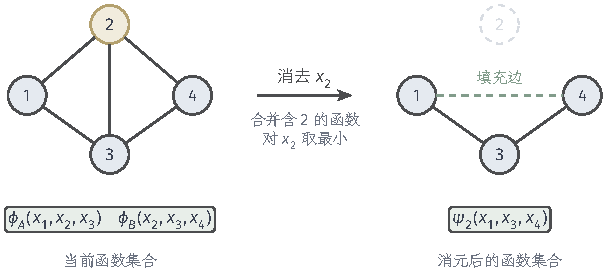
\includegraphics[width=102.687mm]{figures/01-basic-mathematics/04-graphs/tikz/c5-elimination-step/figure.pdf}
  \caption{消去$x_2$时的函数更新与图更新。左：消元前，黄色的$x_2$同时属于$\phi_A$与$\phi_B$的作用域，它的邻居是$1,3,4$。右：消元后，两个函数被新函数$\psi_2(x_1,x_3,x_4)$取代，$x_2$及其关联边被删除，邻居$1,3,4$两两相邻，其中绿色虚线$\{1,4\}$是填充边。}
  \label{fig:graph-dp-elimination-step}
\end{figure}

一般地，消元在原始图上对应一个纯粹的结构操作：把$i$的当前邻居两两连边，然后删去$i$及其关联边。不含$i$的函数提供的边保持不变；含$i$的函数在剩余变量之间提供的边都落在$R_i$内，已被补成的团覆盖。因此，消元后函数集合的原始图恰好是对原始图执行这一操作的结果。

\paragraph{数值计算与结构记账}
图上的操作只预测新函数可能同时读取哪些变量，不计算新函数的取值。对特殊的局部函数，新函数可能仍能进一步分解。例如，若$\phi_A(x_1,x_2,x_3)=g(x_1)+h(x_2,x_3)$，则
\[
\psi_2(x_1,x_3,x_4)=g(x_1)+\min_{x_2}\bigl[h(x_2,x_3)+\phi_B(x_2,x_3,x_4)\bigr],
\]
它是一个$x_1$的函数与一个$(x_3,x_4)$的函数之和，实际上并不需要同时索引$x_1$与$x_4$。图上的填充边不知道这种数值巧合，所以补边图给出的是通用情形下的作用域上界。后面讨论树分解时只使用这种结构记账：它适用于作用域给定、函数值任意的全部问题；具体函数是否还能化简，要回到数值表本身判断。

\subsection{消元次序与计算开销}

定理~\ref{thm:graph-dp-elimination}允许任意消元次序，不同次序给出相同的最优值，但中间函数的大小可以相差很多。下面在四变量例子上比较两个\term{消元次序}（elimination order）：$(1,4,2,3)$与$(2,1,3,4)$。

\paragraph{两种次序的逐步对照}
按$(1,4,2,3)$：消去$x_1$得到上面的$\psi_1(x_2,x_3)=(0,0,1,2)$；消去$x_4$时只有$\phi_B$含$4$，得到$\psi_4(x_2,x_3)=\min_{x_4}\phi_B=(1,0,0,1)$；消去$x_2$时合并$\psi_1,\psi_4$，得到只依赖$x_3$的表（记为$\psi_2'$，以区别于上面先消$x_2$时的$\psi_2$）$\psi_2'(x_3)=\bigl(\min(0+1,1+0),\ \min(0+0,2+1)\bigr)=(1,0)$；最后消去$x_3$得常数$0$。

按$(2,1,3,4)$消元时，第一步就要在$x_1,x_3,x_4$的$8$种取值下各比较$x_2$的两种状态，得到$8$项的$\psi_2$；其后得到的表依次为$(x_3,x_4)$上的$(2,1,0,4)$、$x_4$上的$(0,1)$，最后同样得常数$0$。表~\ref{tab:graph-dp-elimination-orders}列出了每一步的作用域和规模，图~\ref{fig:graph-dp-elimination-orders}画出了对应的图变化。

\begin{table}[!htb]
  \centering
  \caption{四变量例子上两种消元次序的逐步规模。“枚举”指计算新函数时要比较的候选组合数，即$R_i\cup\{i\}$上的配置数；“输出”指新函数表的项数，回溯表的项数与之相同。}
  \label{tab:graph-dp-elimination-orders}
  \begin{tabular}{cccccccc}
    \toprule
    \multicolumn{4}{c}{次序$(1,4,2,3)$} & \multicolumn{4}{c}{次序$(2,1,3,4)$}\\
    \cmidrule(lr){1-4}\cmidrule(lr){5-8}
    消去 & 新作用域 & 枚举 & 输出 & 消去 & 新作用域 & 枚举 & 输出\\
    \midrule
    $x_1$ & $\{2,3\}$ & $8$ & $4$ & $x_2$ & $\{1,3,4\}$ & $16$ & $8$\\
    $x_4$ & $\{2,3\}$ & $8$ & $4$ & $x_1$ & $\{3,4\}$ & $8$ & $4$\\
    $x_2$ & $\{3\}$ & $4$ & $2$ & $x_3$ & $\{4\}$ & $4$ & $2$\\
    $x_3$ & $\varnothing$ & $2$ & $1$ & $x_4$ & $\varnothing$ & $2$ & $1$\\
    \midrule
    合计 & & $22$ & $11$ & 合计 & & $30$ & $15$\\
    \bottomrule
  \end{tabular}
\end{table}

\begin{figure}[!htb]
  \centering
  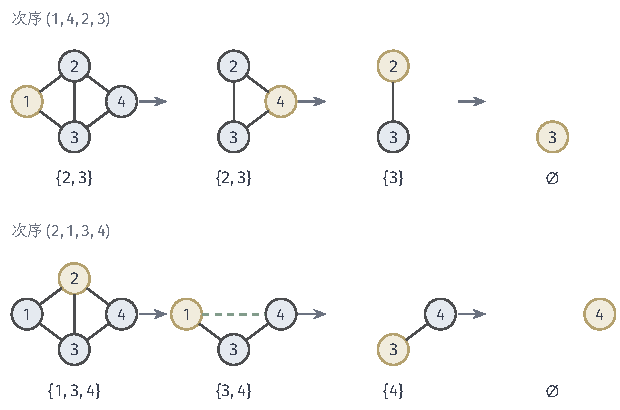
\includegraphics[width=105.004mm]{figures/01-basic-mathematics/04-graphs/tikz/c5-elimination-orders/figure.pdf}
  \caption{两种消元次序下原始图的变化。上行按$(1,4,2,3)$消元，每一步被消去的黄色顶点的邻居都已两两相邻，不产生填充边，新函数至多读取两个变量。下行按$(2,1,3,4)$消元，消去$2$时要补入填充边$\{1,4\}$（第二个图中的绿色虚线），新函数读取三个变量。每个图下方标出消去黄色顶点后新函数的作用域。}
  \label{fig:graph-dp-elimination-orders}
\end{figure}

两种次序都正确，也都恢复出同一个最优配置：$x_1=0$，$x_2=0$，$x_3=1$，$x_4=0$，代回表~\ref{tab:graph-dp-ternary-tables}得$\phi_A(0,0,1)+\phi_B(0,1,0)=0+0=0$。差别在于规模：第一种次序的最大中间表只有$4$项，第二种有$8$项。在这个小例子里差别不大；但若每个变量有$q$个状态，读取$r$个变量的表就有$q^r$项，多读取一个变量意味着表扩大$q$倍。

\paragraph{每一步的开销}
设消去$x_i$时$|R_i|=r_i$，各变量至多$q$个状态。计算$\psi_i$要对$R_i\cup\{i\}$的至多$q^{r_i+1}$种取值，各读取$\mathcal F_i$中每个函数一次，时间约为$|\mathcal F_i|\,q^{r_i+1}$；输出表与回溯表各至多$q^{r_i}$项。整个消元的时间由各步之和给出，主导项来自$r_i$最大的那一步。查找含$i$的函数还需要按变量维护的函数索引，这部分开销与函数个数成正比。

所以变量消元的规模取决于“最多同时处理多少个变量”，即$\max_i(r_i+1)$。这个数由依赖图和消元次序共同决定：有限状态并不保证精确消元总是可行，在某些图上，无论怎样排序，都会有一步需要同时处理很多变量。下一节用树分解描述这些同时处理的变量组，并用树宽给出与次序无关的结构度量。
